\section{Deep Learning}\label{sec:deep-learning}

Deep learning method is part of machine learning methods based on artificial neural network with representation learning.
The learning process can be supervised, semi-supervised, or unsupervised.

There is a very large variety of deep learning architectures, some of them are specialized in some fields meanwhile others have a broader usage, especially, there are CNNs and Transformers.

In recent years, the field of computer vision has been growing in complexity and the number of applications has been increasing, in addition to those presented in \hyperref[sec:background]{Section 1.1 Computer vision}, there are \gls{slam} and visual odometry which is a task in which the robot is able to understand where it is and how it is oriented.

The development of computer vision has been a long process, the growth is favoured by the development of new hardware components and new challenges, about the latters, we have
CIFAR-10 (Doon et al.~\cite{cifar10_paper}), Fashion-MNIST(Xiao et al.~\cite{fashion_mnist_paper}), MS-Coco (Lin et al.~\cite{ms_coco_paper}) and ImageNet (Deng et al.~\cite{imagenet_paper}).
These datasets are often used as benchmark for novel approaches.

For the architectures, starting from AlexNet (Krizhevsky et al.~\cite{alex_net_paper}), then VGG (Simonyan et al.~\cite{vgg_paper}), Inception-V1 (Szegedy et al.~\cite{inception_v1_paper}), Inception-V2 (Szegedy et al.~\cite{inception_v2_paper}), ResNet (He et al.~\cite{resnet_paper}), etc., the complexity of the models has increased enormously.
Each of these models introduced some innovations and improved the performance on the benchmarks, for example:
\begin{itemize}
    \item AlexNet introduced the concept of the \emph{convolutional neural network} (CNN) and use of the separation of the models into two different GPUs.
    \item VGG introduced the concept of stage, which repeated more times, composes the model.
    \item Inception-V1, Inception-V2 and Inception-V3 which are based on the concept of \emph{inception module} which was composed by different paths that the input has to go through to reach the output.
    \begin{figure}[H]
        \centering
        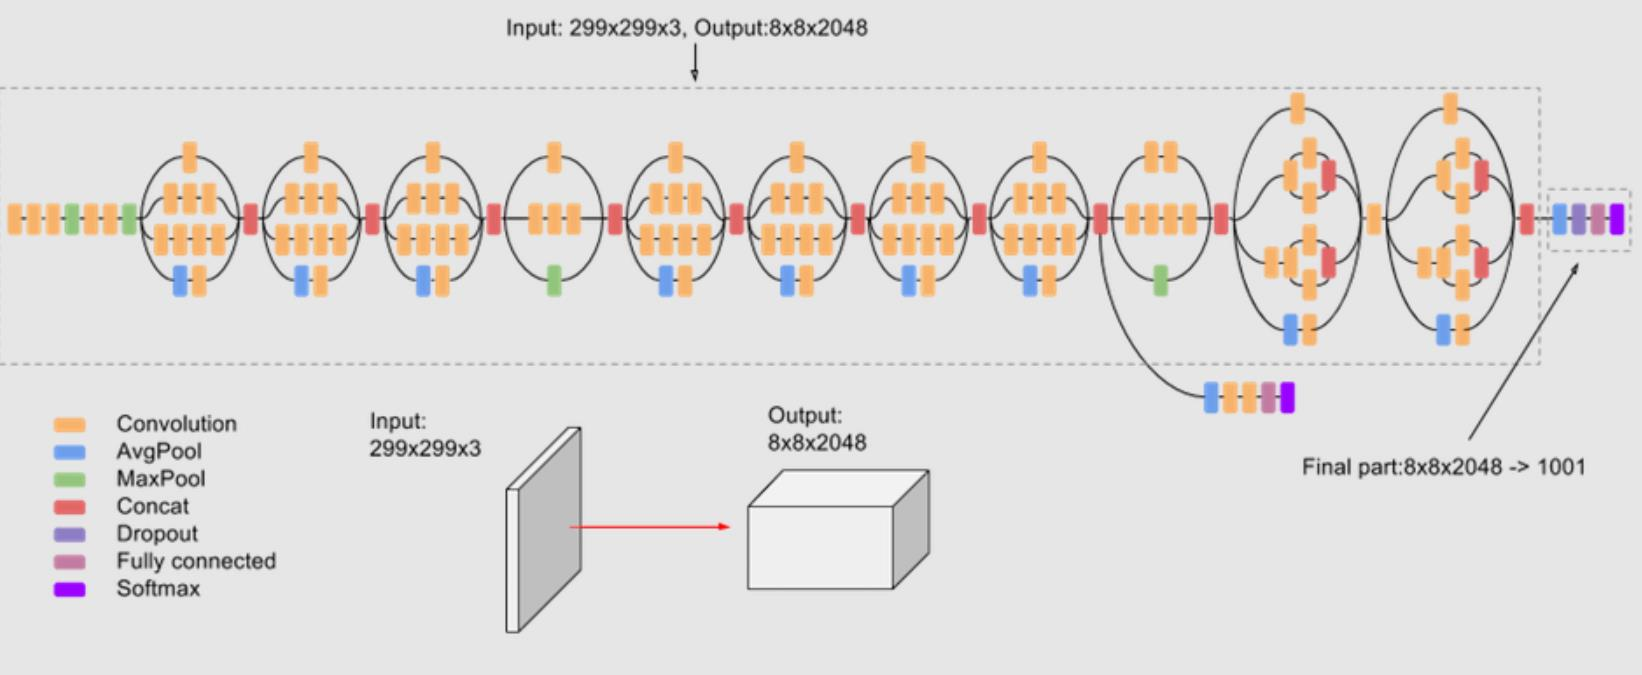
\includegraphics[width=\textwidth]{images/2_inception_v3}
        \caption{Inception V3 Structure.}\label{fig:inception-v3}
    \end{figure}
    \item ResNet is a model that is based on the concept of \emph{residual network} which is composed by several blocks of the same type with the skip connections:
    \begin{figure}[H]
        \centering
        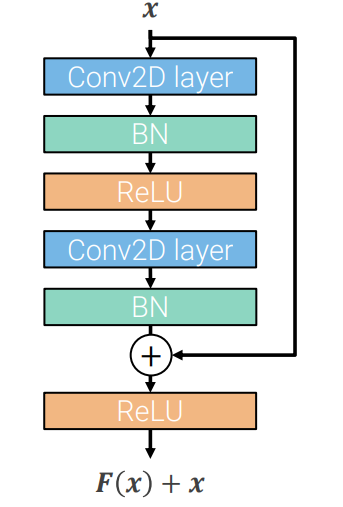
\includegraphics[width=0.4\textwidth]{images/2_1_skip_connection}
        \caption{Skip connection.}\label{fig:skip-connection}
    \end{figure}
    Basically, the input of the block is added to the output before feeding it to the next block, in this way, we can avoid the \gls{vanishing gradient problem} making easier the training process.
\end{itemize}
After this, the computer-visionists lend the Transformer architecture (Vaswani et al.~\cite{transformer_paper}) from \gls{nlp}, bringing up ViT (Dosovitskiy et al.~\cite{vit_paper}) which is based on the \gls{mha} mechanism.
A multi-head attention is a module of attention mechanisms repeated several times in parallel.
In this way, the model can attend to different parts of the input, forming the cross-attention over different parts of the input.
For major details, please refer to \hyperref[subsec:transformer]{\S2.1.2 Transformer}.


\subsection[CNN]{Convolutional Neural Network}\label{subsec:conv-neural-network}
The \gls{cnn} is a class of artificial neural network, it is used in almost every imagery related task, such as image classification, object detection, image segmentation, etc.

The CNN takes an input image, assign importance (learnable weights and biases) and process the input image by using the convolution operation extracting features.
There are two important parameters in the convolution operation, the kernel size and the stride.
The kernel is a matrix which is used to perform the convolution operation, the stride is the number of pixels the kernel slides each step over the input image to produce a new pixel of the output feature map.
With stride, we can control the size of the output image, if the stride is equal to 1, the output image will have the same size of the input image, if the stride is equal to 2, the output image will have half the size of the input image.
\begin{figure}[H]
    \centering
    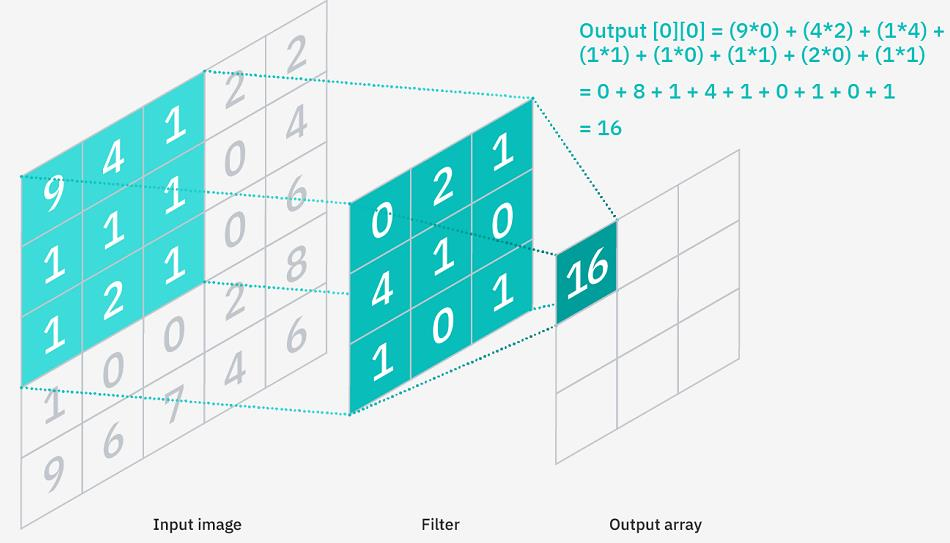
\includegraphics[width=\textwidth]{images/2_convolutions}
    \caption[Example of convolution]{Convolutions: every single element of the output feature map is obtained by summing the element-wise product between the elements from the input feature map and the kernel. The whole feature map is then obtained sliding the kernel over the input feature map.}
    \label{fig:figure-convolutions}
\end{figure}
Then, there are pooling layers, usually max-pooling and average pooling, which can reduce the dimensionality of the feature maps by setting strides $>=2$, which is useful to reduce the computational cost.
An important property of max-pooling is that it is translation invariant, which means that the output of the max-pooling layer is the same regardless of the position of the input feature map.
For example, max-pooling is computed as showed in the image:
\begin{figure}[H]
    \centering
    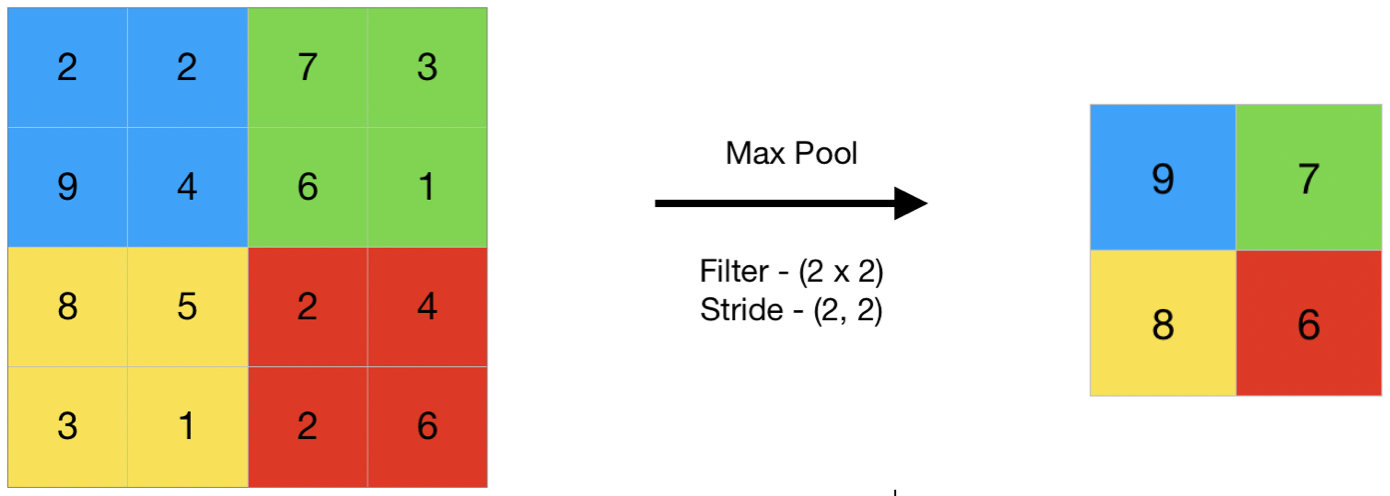
\includegraphics[width=\textwidth]{images/2_max_pooling}
    \caption[Example of max-pooling]{Max-pooling: essentially, it strides over the input image and takes the max value of the area covered by the kernel.}
    \label{fig:figure-max-pooling}
\end{figure}
With stride = 2, sliding over the input feature map and taking the maximum value of the window, the dimensionality of the feature map is reduced.

Another important component is the activation function, \gls{relu} is the most used one, it is defined as:
\begin{equation}
    ReLU(x) = \max(0, x)
    \label{eq:expression-relu}
\end{equation}
It guarantees the non-linearity of the network, allowing the network to learn more complex features.
These are the main components of a CNN, but there are other components, such as batch normalization and dropout which are used to improve the performance of the network reducing the over-fitting.
Increasing the number of layers and combining the pooling layers, the CNN is able to extract more and more complex features, such as edges, lines, shapes, etc.
Currently, the most used CNN architecture is the ResNet which will be used in the project as feature-extractor.

\subsection{Transformer}\label{subsec:transformer}
The transformer architecture is a class of neural network architecture, born for the task of machine translation, but it has been used in many vision tasks.

As introduced in ~\cite{transformer_paper}, the Transformer is a model architecture based entirely on attention mechanism.
Which can be divided into different steps: the first step of attention mechanism is to compute the Q, K and V vectors, by multiplying the input vector $x$ by the weight matrices $W_q$, $W_k$ and $W_v$.
Then, the attention weights are computed by using the scaled dot product attention, which is the softmax of the dot product between the query and the key vectors divided by the square root of the dimensionality of the key vector.
Finally, the attention weights are multiplied by the value vector to obtain the output vector.
The output vector is then passed through a feed-forward neural network, which is composed by two linear layers with ReLU activation function, added to the input vector and normalized by the layer normalization.
The self-attention module is then repeated $N$ times, where $N$ is the number of layers.

The whole process can be summarized as the:
\begin{equation}
    Attention(Q, K, V) = softmax\left(\frac{QK^T}{\sqrt{d_k}}\right)V
    \label{eq:expression-scaled-dot-product}
\end{equation}
And the graphical representation is:

\begin{figure}[H]
    \centering
    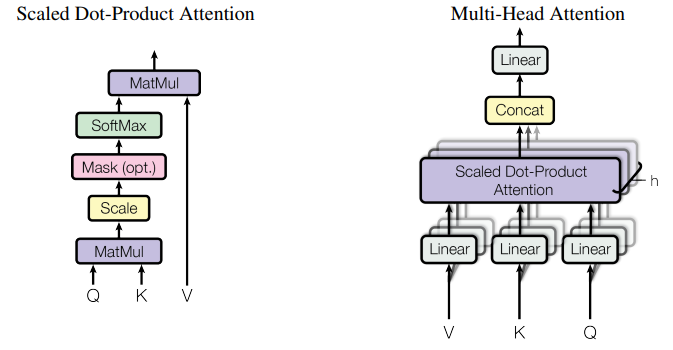
\includegraphics[width=\textwidth]{./images/2_attention}
    \caption[Attention mechanisms]{Attention mechanism: (Left) scaled-dot-product attention. (right) Multi-head attention which is obtained by combining many scaled-dot-product attention.}
    \label{fig:figure-encoder-structure}
\end{figure}

An important notion introduced is the multi-head attention, which is using more scaled dot product attention, each one with different weights, and concatenating each output vectors.
And this is the transformer encoder.

Then, using a slightly modified version of the self-attention module, we obtain the decoder, which takes as input also the output sequence from encoder, and repeating the number of encoder and decoder modules, we obtain the whole transformer architecture, as follows:

\begin{figure}[H]
    \centering
    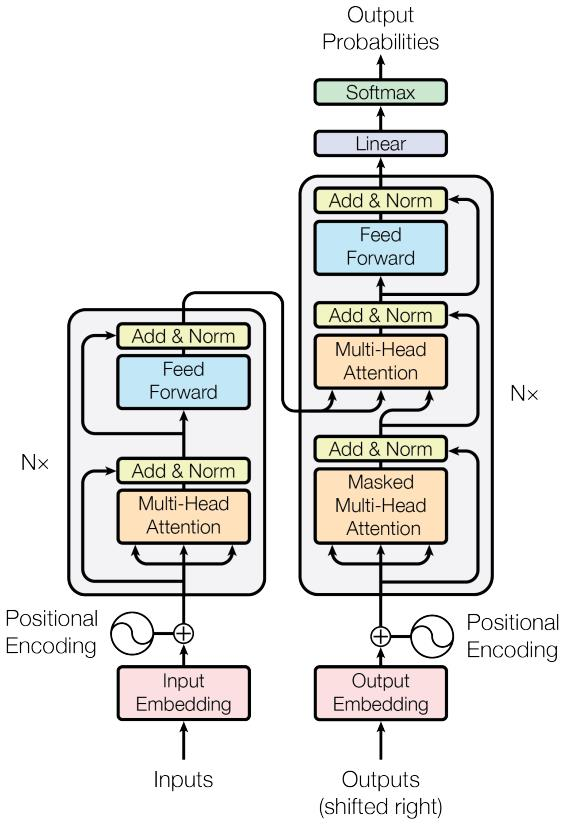
\includegraphics[width=0.7\textwidth]{./images/2_transformer}
    \caption[Transformer architecture]{Transformer architecture: the encoder and decoder modules are composed by a self-attention module and a feed-forward neural network repeated $N$ times.}
    \label{fig:figure-transformer-architecture}
\end{figure}

With this architecture the new state-of-the-art results have been achieved in Natural Language Processing, especially in machine translation (a \gls{seq2seq} task).
Then the adapted version applied to vision tasks also brought very good results, such as in object detection, image captioning, etc.

Another important notion is the mask which is used in sequence-to-sequence models, such as the transformer more specifically in the decoder, to avoid the model to attend to the future tokens.
To ensure this, the future positions are masked with $-\infty$ before the softmax step in the self-attention calculation.